% -----------------------------------------------
% Template for SMC 2023
% based on SMC 2022 template
% -----------------------------------------------

\documentclass{article}
\usepackage{smc}
\usepackage{times}
\usepackage{ifpdf}
\usepackage[english]{babel}
\usepackage{cite}

%%%%%%%%%%%%%%%%%%%%%%%% Some useful packages %%%%%%%%%%%%%%%%%%%%%%%%%%%%%%%
%%%%%%%%%%%%%%%%%%%%%%%% See related documentation %%%%%%%%%%%%%%%%%%%%%%%%%%
%\usepackage{amsmath} % popular packages from Am. Math. Soc. Please use the 
%\usepackage{amssymb} % related math environments (split, subequation, cases,
%\usepackage{amsfonts}% multline, etc.)
%\usepackage{bm}      % Bold Math package, defines the command \bf{}
%\usepackage{paralist}% extended list environments
%%subfig.sty is the modern replacement for subfigure.sty. However, subfig.sty 
%%requires and automatically loads caption.sty which overrides class handling 
%%of captions. To prevent this problem, preload caption.sty with caption=false 
%\usepackage[caption=false]{caption}
%\usepackage[font=footnotesize]{subfig}


%user defined variables
\def\papertitle{Natural Language Processing: Does it work like our brain?}
\def\firstauthor{Luis Miguel Garcia Marin}
\def\secondauthor{Second author}
\def\thirdauthor{Third author}

% adds the automatic
% Saves a lot of output space in PDF... after conversion with the distiller
% Delete if you cannot get PS fonts working on your system.

% pdf-tex settings: detect automatically if run by latex or pdflatex
\newif\ifpdf
\ifx\pdfoutput\relax
\else
   \ifcase\pdfoutput
      \pdffalse
   \else
      \pdftrue
\fi

\ifpdf % compiling with pdflatex
  \usepackage[pdftex,
    pdfauthor={\firstauthor, \secondauthor, \thirdauthor},
    bookmarksnumbered, % use section numbers with bookmarks
    pdfstartview=XYZ % start with zoom=100% instead of full screen; 
                     % especially useful if working with a big screen :-)
   ]{hyperref}
  %\pdfcompresslevel=9

  \usepackage[pdftex]{graphicx}
  % declare the path(s) where your graphic files are and their extensions so 
  %you won't have to specify these with every instance of \includegraphics
  \graphicspath{{./figures/}}
  \DeclareGraphicsExtensions{.pdf,.jpeg,.png}

  \usepackage[figure,table]{hypcap}

\else % compiling with latex
  \usepackage[dvips,
    bookmarksnumbered, % use section numbers with bookmarks
    pdfstartview=XYZ % start with zoom=100% instead of full screen
  ]{hyperref}  % hyperrefs are active in the pdf file after conversion

  \usepackage[dvips]{epsfig,graphicx}
  % declare the path(s) where your graphic files are and their extensions so 
  %you won't have to specify these with every instance of \includegraphics
  \graphicspath{{./figures/}}
  \DeclareGraphicsExtensions{.eps}

  \usepackage[figure,table]{hypcap}
\fi

%setup the hyperref package - make the links black without a surrounding frame
\hypersetup{
    colorlinks,%
    citecolor=black,%
    filecolor=black,%
    linkcolor=black,%
    urlcolor=black
}


% Title.
% ------
\title{\papertitle}

% Authors
% Please note that submissions are NOT anonymous, therefore 
% authors' names have to be VISIBLE in your manuscript. 
%
% Single address
% To use with only one author or several with the same address
% ---------------
%\oneauthor
%   {\firstauthor} {Affiliation1 \\ %
%     {\tt \href{mailto:author1@smcnetwork.org}{author1@smcnetwork.org}}}

%Two addresses
%--------------
% \twoauthors
%   {\firstauthor} {Affiliation1 \\ %
%     {\tt \href{mailto:author1@smcnetwork.org}{author1@smcnetwork.org}}}
%   {\secondauthor} {Affiliation2 \\ %
%     {\tt \href{mailto:author2@smcnetwork.org}{author2@smcnetwork.org}}}

% Three addresses
% --------------
 \oneauthor
   {\firstauthor} {Fulda University of Applied Science \\ %
     {\tt \href{mailto:luis-miguel.garcia-marin@informatik.hs-fulda.de}{luis-miguel.garcia-marin@informatik.hs-fulda.de}}}


% ***************************************** the document starts here ***************
\begin{document}
%
\capstartfalse
\maketitle
\capstarttrue

\tableofcontents

%
\begin{abstract}
In this paper we introduce ourselves into the Natural Language Processing (NLP) world, and we discuss if it is possible to understand the functioning of the new discovered technics in NLP with our understanding on the functioning of our brain with its habitual processing of natural language. And in order to do it, it is used a variety of inputs like brain image records with some recent models in Deep Learning.
\end{abstract}
%

\section{Introduction}\label{sec:introduction}

\subsection{How everything started}
At the ACL Conference in 1987, Don Walker, Jane Robinson and Karen Spark Jones were talking about when NLP research began\cite{jones1994natural}. Fred Thompson said that he began in 1954 and others, like Martin Key, started out too in the 50's. Work in the field has concentrated first on one problem, then on another, sometimes because solving problem X depends on solving problem Y, but sometimes just because problem Y seems more tractable than problem X. This means that the focus was not to solve NLP the same way that our brain does, because this was not tractable, so the problems were tried to solve in a lexico-logical way at first. 
\subsection{Nowadays}
This triggered that NLP has been traditionally a complex problem to solve\cite{jones1992natural}. However, Recurrent Neural Networks and two significant advances - one in 2017 and another in 2019 - brought substantial improvements to NLP. In 2017, a new form of deep learning model called Transformer\cite{wang2019r} made it possible to parallelize ML training more efficiently, resulting in vastly improved accuracies.
In 2019, Google introduced Bidirectional Encoder Representations from Transformers (BERT)\cite{kamath2022bidirectional}, which improves the above Transformer architecture. Straightaway BERT helped achieve state-of-the-art performance\cite{DBLP:journals/corr/abs-1810-04805} on several NLP tasks such as reading comprehension, text extraction, sentiment analysis, etc. These two advancements meant that NLP could easily outdo average humans in many tasks and in some cases, even exceed the performance of subject matter experts. 
\subsection{Our question}
But does recurrent neural network propagation of information works similar as our brain does? We propose to look at brain activity of subjects reading naturalistic text as a source of additional information for interpreting neural networks. And to do this we use brain imaging recordings of subjects reading complex natural text to interpret word and sequence embeddings from 4 recent NLP models - ELMo, USE, BERT and Transformer-XL, and study how their representations differ across layer depth, context length, and attention type.

\section{State of the Art}
\label{sec:state_of_the_art}

Most work investigating language in the brain has been done in a controlled experiment setup where two conditions are contrasted\cite{friederici2011brain}. These conditions typically vary in complexity (simple vs. complex sentences), in the presence or absence of a linguistic property (sentences vs. lists of words) or in the presence or absence of incongruities (e.g. semantic surprisal)\cite{friederici2011brain}. A few researchers instead use naturalistic stimulus such as stories\cite{brennan2012syntactic}. Some use predictive models of brain activity as a function of multi-dimensional features spaces describing the different properties of the stimulus\cite{wehbe2014simultaneously}.

A few previous works have used neural network representations as a source of feature spaces to model brain activity. Wehbe et al.\cite{wehbe2014simultaneously} aligned the MEG brain activity we use here with a Recurrent Neural Network (RNN), trained on an online archive of Harry Potter Fan Fiction. The authors aligned brain activity with the context vector and the word embedding, allowing them to trace sentence comprehension at a word-by-word level. Jain and Huth\cite{jain2018incorporating} aligned layers from a Long Short-Term Memory (LSTM) model to fMRI recordings of subjects listening to stories to differentiate between the amount of context maintained by each brain region. Other approaches rely on computing surprisal or cognitive load metrics using neural networks to identify processing effort in the brain, instead of aligning entire representations\cite{frank2015erp}.

There is also a little work that evaluates or improves NLP models through brain recordings. Søgaard\cite{sogaard2016evaluating} proposes to evaluate whether a word embedding contains cognition-relevant semantics by measuring how well they predict eye tracking data and fMRI recordings. Fyshe et al.\cite{fyshe2014interpretable} build a non-negative sparse embedding for individual words by constraining the embedding to also predict brain activity well and show that the new embeddings better align with behavioral measures of semantics.


\section{Methodology}\label{sec:methodology}

We investigate how the representations of all four networks (ELMO, BERT, USE and T-XL) change as we provide varying lengths of context. We compute the representations x in each available intermediate layer ([1, 2] for ELMo; [1, 12] for BERT; the layer is the output embedding for USE; and [1, 19] for T-XL). We compute x for word w by passing the most recent k words through the network.

\subsection{fMRI and MEG data} 
We use fMRI and MEG data which complement each other very well. fMRI is sensitive to the change in oxygen level in the blood which is a consequence to neural activity, it has high spatial resolution (2-3 mm) and low temporal resolution (multiple seconds). MEG measures the change in the magnetic field outside the skull due to neural activity, it has low spatial resolution (multiple cm) and high temporal resolution (up to 1KHz). We use fMRI data published by Wehbe et al.\cite{wehbe2014simultaneously}: 8 subjects read chapter 9 of Harry Potter and the Sorcerer’s stone\cite{rowling2012harry} which was presented one word at a time for a fixed duration of 0.5 seconds each, and 45 minutes of data were recorded. The fMRI sampling rate (TR) was 2 seconds. The same chapter was shown by Wehbe et al.\cite{wehbe2014aligning} to 3 subjects in MEG with the same rate of 0.5 seconds per word. Details about the data and preprocessing can be found in the supplementary materials.

\subsection{Encoding models} 
For each type of network-derived representation x, we estimate an encoding model that takes x as input and predicts the brain recording associated with reading the same k words that were used to derive x. We estimate a function f, such that f(x) = y, where y is the brain activity recorded with either MEG or fMRI. We follow previous work\cite{wehbe2014simultaneously} and model f as a linear function, regularized by the ridge penalty. The model is trained via four-fold cross-validation and the regularization parameter is chosen via nested cross-validation.

\subsection{Evaluation of predictions}
We evaluate the predictions from each encoding model by using them in
a classification task on held-out data, in the four-fold cross-validation setting. The classification task is to predict which of two sets of words was being read based on the respective feature representations of these words\cite{wehbe2014simultaneously,wehbe2014aligning}. This task is performed between sets of 20 consecutive TRs in fMRI (accounting for the slowness of the hemodynamic response), and sets of 20 randomly sampled words in MEG. The classification is repeated a large number of times and an average classification accuracy is obtained for each voxel in fMRI and for each sensor/timepoint in MEG. We refer to this accuracy of matching the predictions of an encoding model to the correct brain recordings as "prediction accuracy". The final fMRI results are reported on the MNI template, and we use pycortex to visualize them\cite{gao2015pycortex}. 

\begin{figure}[t]
\centering
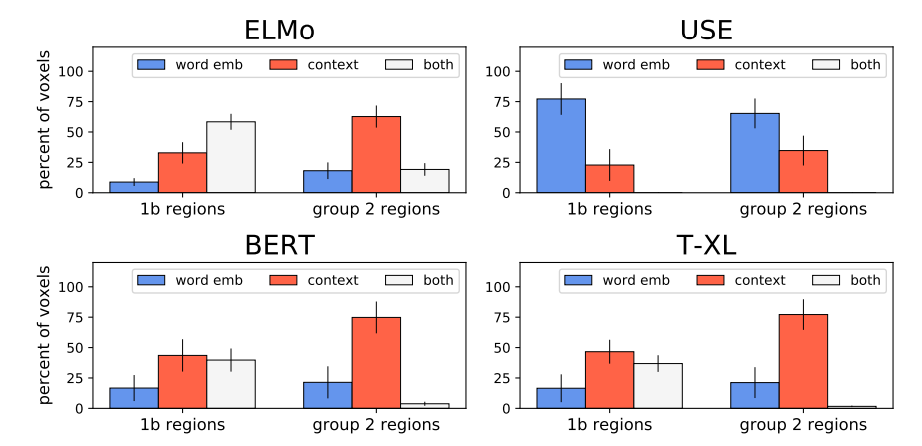
\includegraphics[width=1.1\columnwidth]{pycortex.png}
\caption{Amount of group 1b regions and group 2 regions predicted well by each network-derived representation: a 10-word representation corresponding to the 10 most recent words shown to the participant (Red) and a word-embedding corresponding to the last word (Blue). White indicates that both representations predict the specified amount of the regions well (about 0.7 threshold).\label{fig:pycortex}}
\end{figure}

\subsection{Proof of concept}
Since MEG signals are faster than the rate of word presentation, they are more
appropriate to study the components of word embeddings than the slow fMRI signals that cannot be
attributed to individual words. We know that a word embedding learned from a text corpus is likely to
contain information related to the number of letters and part of speech of a word. We show in section
4 of the supplementary materials that the number of letters of a word and its ELMo embedding
predict a shared portion of brain activity early on (starting 100ms after word onset) in the back of the
MEG helmet, over the visual cortex. Indeed, this region and latency are when we expect the visual
information related to a word to be processed (Sudre et al., 2012). Further, a word’s part of speech
and its ELMo embedding predict a shared portion of brain activity around 200ms after word onset in
the left front of the MEG sensor. Indeed, we know from electrophysiology studies that part of speech
violations incur a response around 200ms after word onset in the frontal lobe (Frank et al., 2015). We
conclude from these experiments that the ELMo embedding contains information about the number
of letters and the part of speech of a word. Since we knew this from the onset, this experiment serves
as a proof of concept for using our approach to interpret information in network representations.


\section{Headings}
First level headings are in Times 12~pt bold, centered with 1 line of space above the section head, and 1/2 space below it.
For a section header immediately followed by a subsection header, the space should be merged.

\subsection{Second Level Headings}
Second level headings are in Times 10~pt bold, flush left, with 1 line of space above the section head, and 1/2 space below it. The first letter of each significant word is capitalized.

\subsubsection{Third Level Headings}
Third level headings are in Times 10~pt italic, flush left, with 1/2 line of space above the section head, and 1/2 space below it. The first letter of significant words is capitalized.

Using more than three levels of headings is strongly discouraged.





\section{Floats and equations}

\subsection{Equations}
Equations should be placed on separated lines and numbered. The number should be on the right side, in parentheses.
\begin{equation}
r=\sqrt[13]{3}
\label{eq:BP}
\end{equation}
Always refer to equations like this: ``Equation (\ref{eq:BP}) is of particular interest because...''

\subsection{Figures, Tables and Captions}
\begin{table}[t]
 \begin{center}
 \begin{tabular}{|l|l|}
  \hline
  String value & Numeric value \\
  \hline
  Hej SMC! & 2023 \\
  \hline
 \end{tabular}
\end{center}
 \caption{Table captions should be placed below the table,  like this.}
 \label{tab:example}
\end{table}

All artwork must be centered, neat, clean and legible. Figures should be centered, neat, clean
and completely legible. All lines should be thick and dark enough for purposes of reproduction. Artwork should not be hand-drawn. The proceedings will be distributed in electronic form only, therefore color figures are allowed. However, you may want to check that your figures are understandable even if they are printed in black-and-white.


Numbers and captions of figures and tables always appear below the figure/table.
Leave 1 line space between the figure or table and the caption.
Figure and tables are numbered consecutively. 
Captions should be Times 10pt. Place tables/figures in the text as close to the reference as possible, 
and preferably at the top of the page.

Always refer to tables and figures in the main text, for example: ``see Fig. \ref{fig:example} and \tabref{tab:example}''.
Figures and tables may extend across both columns to a maximum width of 17.2cm.

Vectorial figures are preferred, e.g., eps. When using \texttt{Matlab}, export using either (encapsulated) Postscript or PDF format. In order to optimize readability, the font size of text within a figure should be no smaller than
that of footnotes (8~pt font-size). If you use bitmap figures, make sure that the resolution is high enough for print quality. 

\begin{figure}[t]
\centering

\includegraphics[width=0.6\columnwidth]{figure}
\caption{Figure captions should be placed below the figure, 
exactly like this.\label{fig:example}}
\end{figure}


\subsection{Footnotes}
You can indicate footnotes with a number in the text \footnote{This is a footnote example.},
but try to work the content into the main text.Use 8~pt font-size for footnotes.  Place the footnotes at the bottom of the page 
on which they appear. Precede the footnote with a 0.5~pt horizontal rule.

\section{Citations}
All bibliographical references should be listed at the end, inside a section named ``REFERENCES''. References must be numbered in order of appearance. You should avoid listing references that do not appear in the text.

Reference numbers in the text should appear within square brackets, such as in~\cite{Someone:00} or~\cite{Someone:00,Someone:04,Someone:09}. The reference format is the standard IEEE one. We highly recommend you use BibTeX 
to generate the reference list.

\section{Conclusions}
Please, submit full-length papers. Submission is fully electronic and automated through the Conference Web Submission System. \underline{Do not} send papers directly by e-mail.


\begin{acknowledgments}
At the end of the Conclusions, acknowledgements to people, projects, funding agencies, etc. can be included after the second-level heading  ``Acknowledgments'' (with no numbering).
\end{acknowledgments} 

%%%%%%%%%%%%%%%%%%%%%%%%%%%%%%%%%%%%%%%%%%%%%%%%%%%%%%%%%%%%%%%%%%%%%%%%%%%%%
%bibliography here
\bibliography{smc2023bib}

\end{document}
